\chapter{Anhang}
Der aktuelle Stand der App auf GitHub: \url{https://github.com/Munzel06/Pfaditechnik} \\

\section{Userstories}

Der Zeitplan in Form von Userstories. Das erste Bild zeigt die Übersicht und die darauf folgenden Bilder zeigen die einzelnen Userstories.

\begin{figure}[!h]
    \centering
    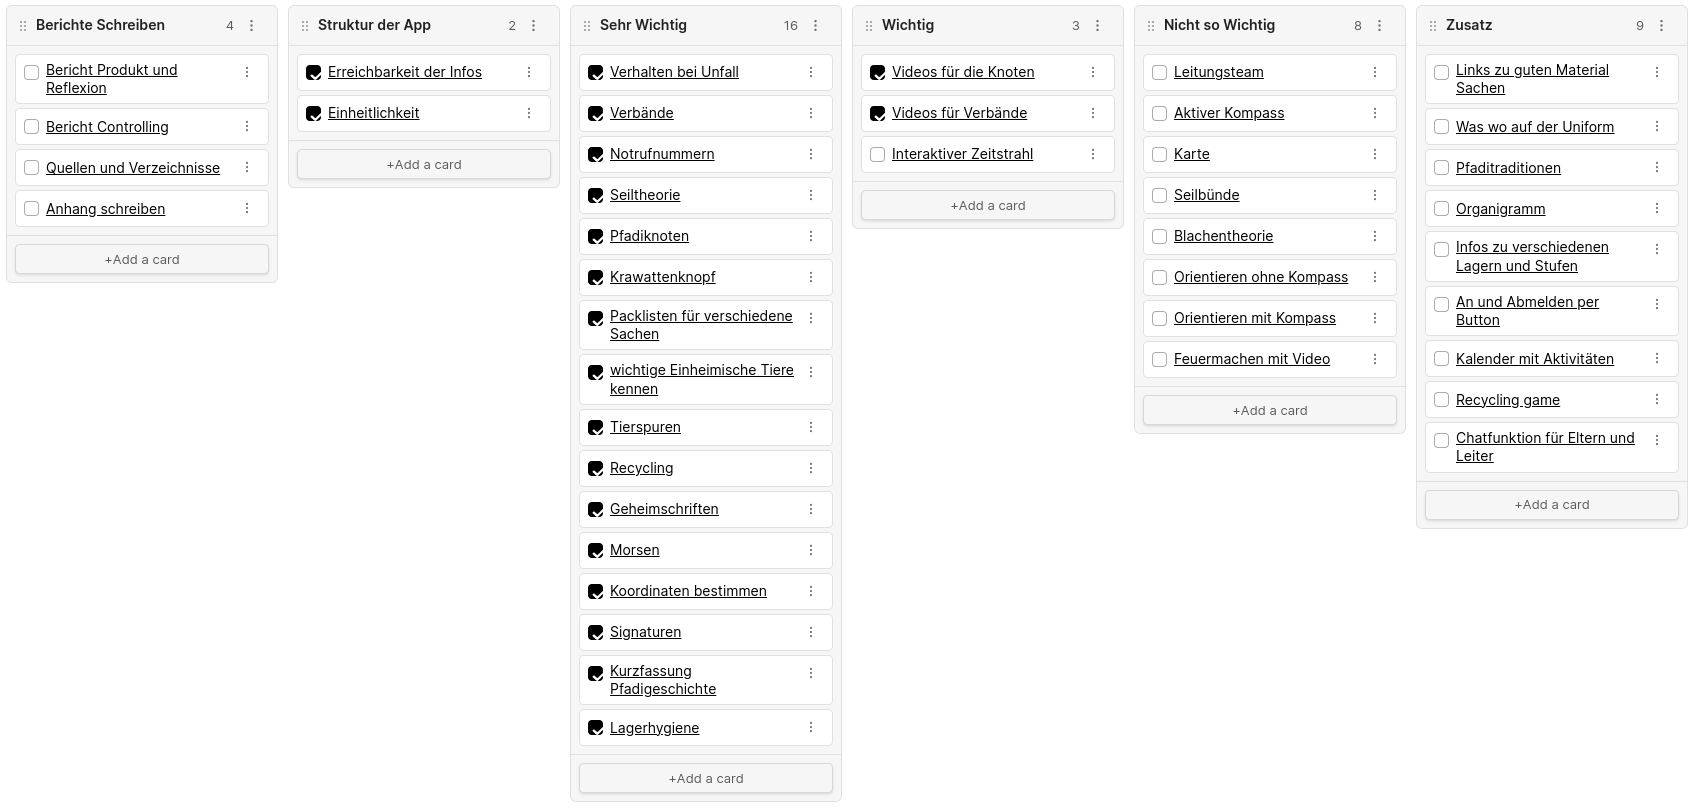
\includegraphics[width=\textwidth]{Picture/overview.png}
    \caption{Übersicht Userstories}
\end{figure}

\begin{table}[ht]
    \centering
    \begin{tabular}{c c}
        \adjustbox{valign=t}{
\includegraphics[width=0.49\textwidth]{Picture/Bericht Produktion Reflexion.png}} &
        \adjustbox{valign=t}{
\includegraphics[width=0.49\textwidth]{Picture/Bericht Controlling.png}} \\
        \vspace{0.01\textwidth} \\
        \adjustbox{valign=t}{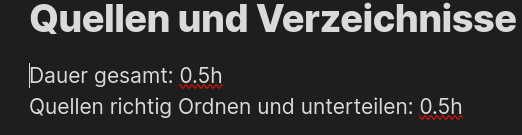
\includegraphics[width=0.49\textwidth]{Picture/Quellen und Verzeichnisse.png}} &
        \adjustbox{valign=t}{
\includegraphics[width=0.49\textwidth]{Picture/Anhang schreiben.png}} \\
        \vspace{0.01\textwidth} \\
        \adjustbox{valign=t}{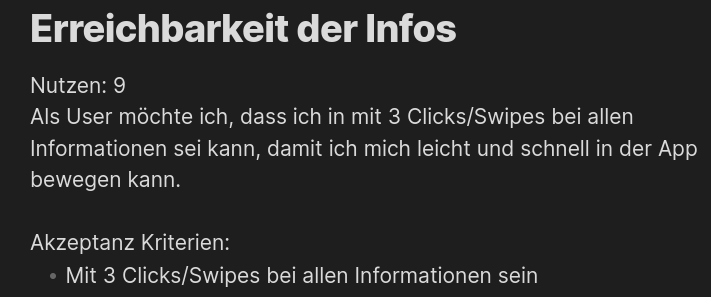
\includegraphics[width=0.49\textwidth]{Picture/Erreichbarkeit der Infos.png}} &
        \adjustbox{valign=t}{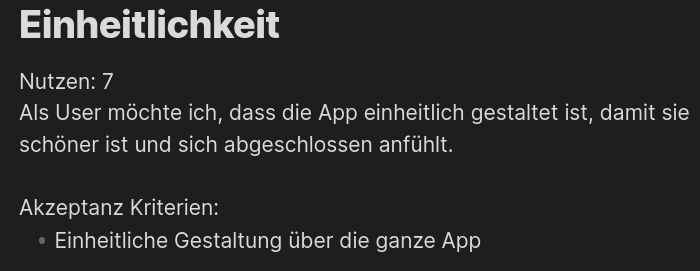
\includegraphics[width=0.49\textwidth]{Picture/Einheitlichkeit.png}} \\
        \vspace{0.01\textwidth} \\
        \adjustbox{valign=t}{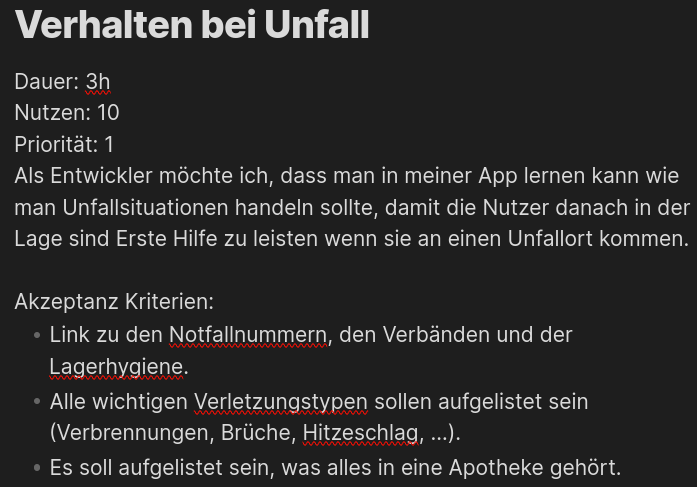
\includegraphics[width=0.49\textwidth]{Picture/Verhalten bei Unfall.png}} &
        \adjustbox{valign=t}{\includegraphics[width=0.49\textwidth]{Picture/Verbände.png}} \\
        \vspace{0.01\textwidth} \\
        \adjustbox{valign=t}{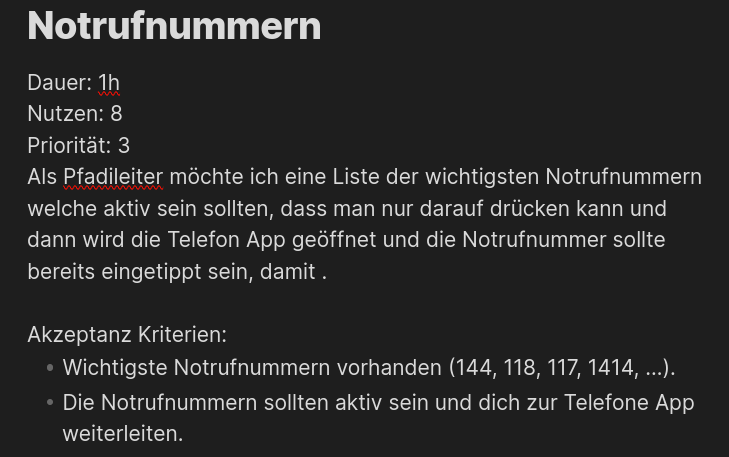
\includegraphics[width=0.49\textwidth]{Picture/Notrufnummern.png}} &
        \adjustbox{valign=t}{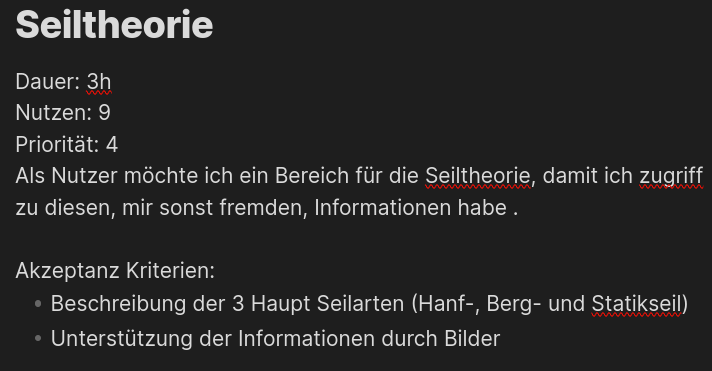
\includegraphics[width=0.49\textwidth]{Picture/Seiltheorie.png}} \\
    \end{tabular}
\end{table}

\begin{table}[ht]
    \centering
    \begin{tabular}{c c}
        \adjustbox{valign=t}{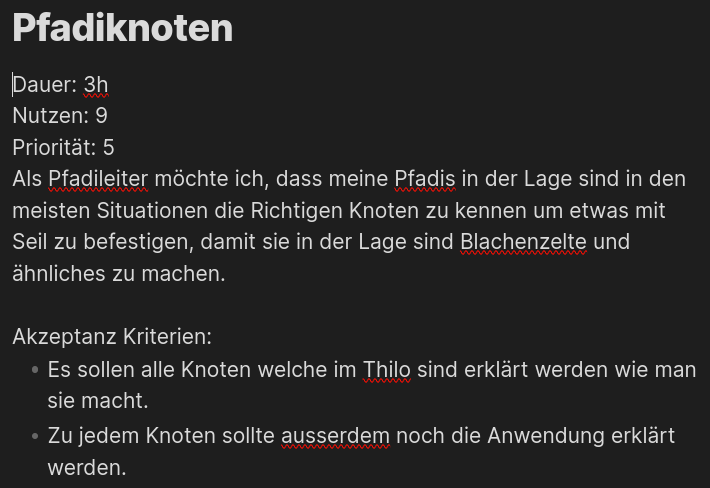
\includegraphics[width=0.49\textwidth]{Picture/Pfadiknoten.png}} &
        \adjustbox{valign=t}{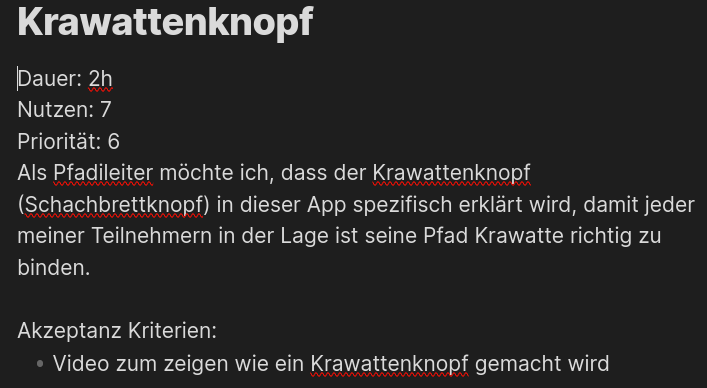
\includegraphics[width=0.49\textwidth]{Picture/Krawattenknoten.png}} \\
        \vspace{0.01\textwidth} \\
        \adjustbox{valign=t}{\includegraphics[width=0.49\textwidth]{Picture/Packlisten für verschiedene Sachen.png}} &
        \adjustbox{valign=t}{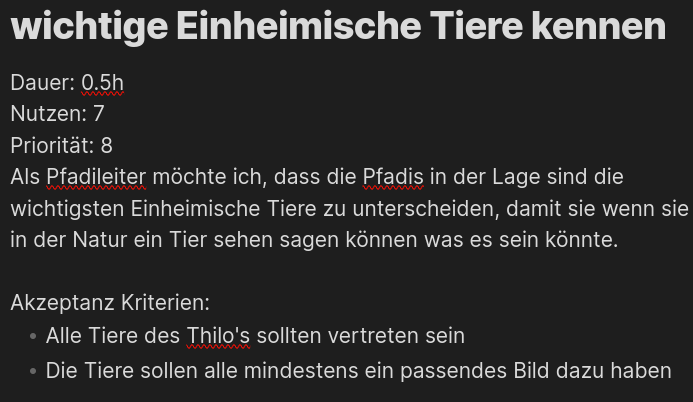
\includegraphics[width=0.49\textwidth]{Picture/wichtige Einheimische Tiere.png}} \\
        \vspace{0.01\textwidth} \\
        \adjustbox{valign=t}{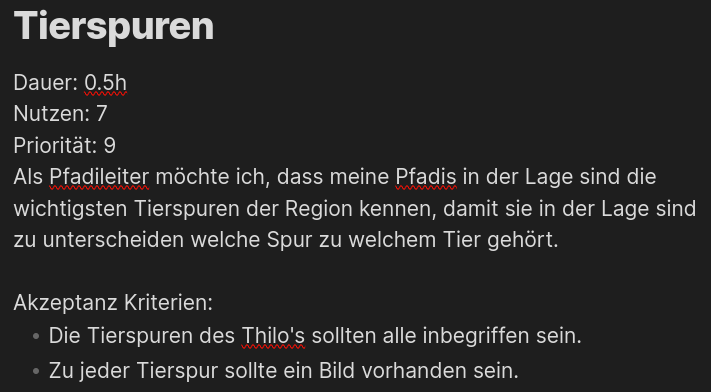
\includegraphics[width=0.49\textwidth]{Picture/Tierspuren.png}} &
        \adjustbox{valign=t}{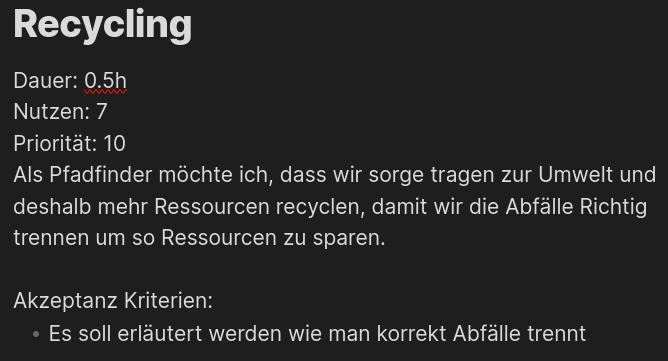
\includegraphics[width=0.49\textwidth]{Picture/Recycling.png}} \\
        \vspace{0.01\textwidth} \\
        \adjustbox{valign=t}{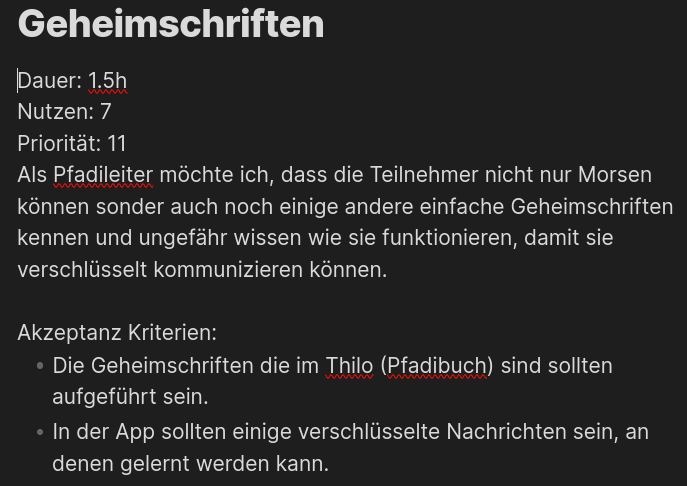
\includegraphics[width=0.49\textwidth]{Picture/Gehmeischriften.png}} &
        \adjustbox{valign=t}{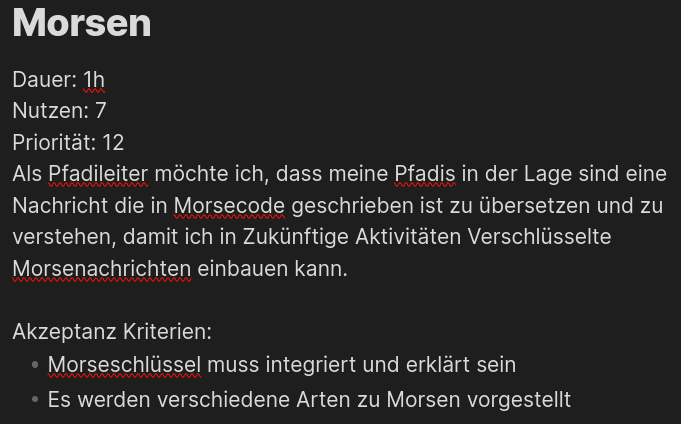
\includegraphics[width=0.49\textwidth]{Picture/Morsen.png}} \\
        \vspace{0.01\textwidth} \\
    \end{tabular}
\end{table}

\begin{table}[ht]
    \centering
    \begin{tabular}{c c}
        \adjustbox{valign=t}{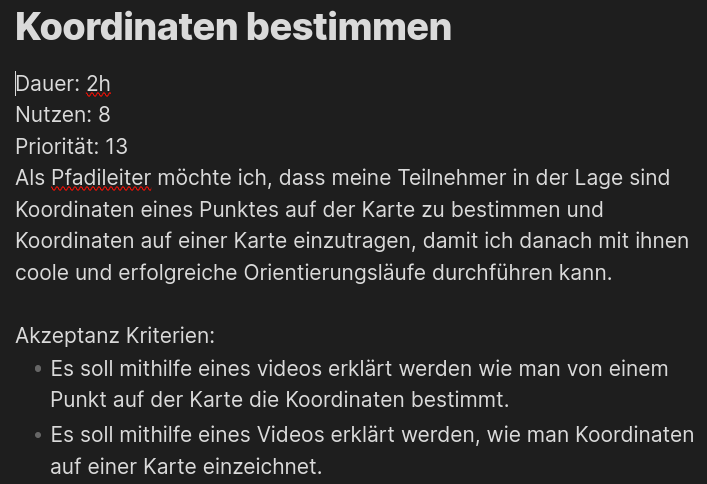
\includegraphics[width=0.49\textwidth]{Picture/Koordinaten bestimmen.png}} &
        \adjustbox{valign=t}{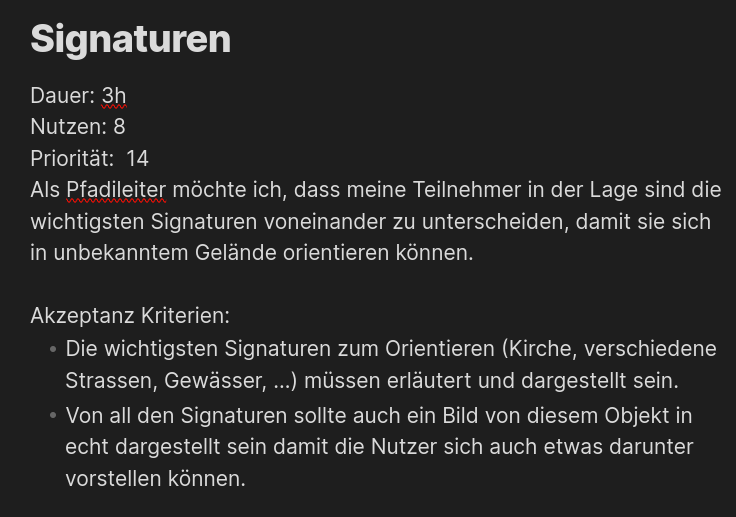
\includegraphics[width=0.49\textwidth]{Picture/Signaturen.png}} \\
        \vspace{0.01\textwidth}\\
        \adjustbox{valign=t}{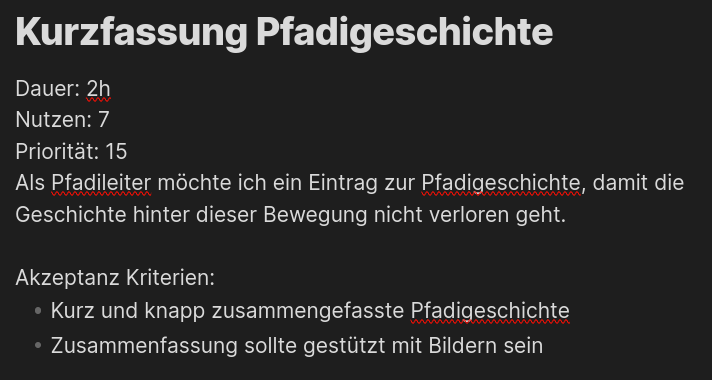
\includegraphics[width=0.49\textwidth]{Picture/Kurzfassung Pfadigeschichte.png}} &
        \adjustbox{valign=t}{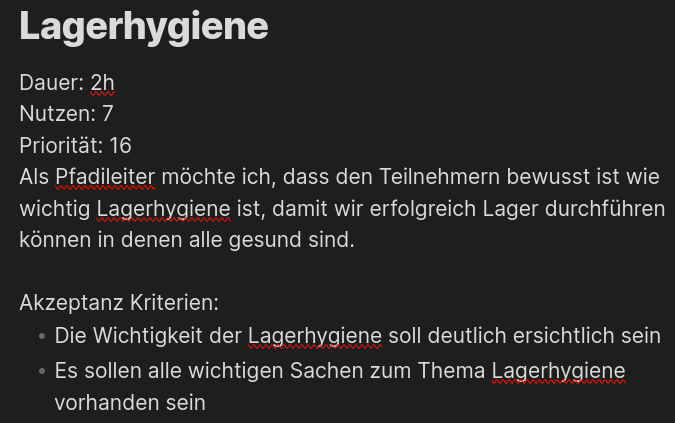
\includegraphics[width=0.49\textwidth]{Picture/Lagerhygiene.png}} \\
        \vspace{0.01\textwidth} \\
        \adjustbox{valign=t}{\includegraphics[width=0.49\textwidth]{Picture/Videos für die Knoten.png}} &
        \adjustbox{valign=t}{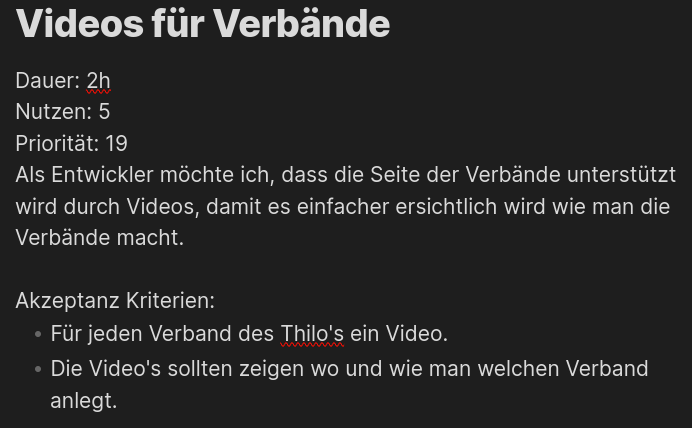
\includegraphics[width=0.49\textwidth]{Picture/Videos für Verbände.png}} \\
        \vspace{0.01\textwidth} \\
        \adjustbox{valign=t}{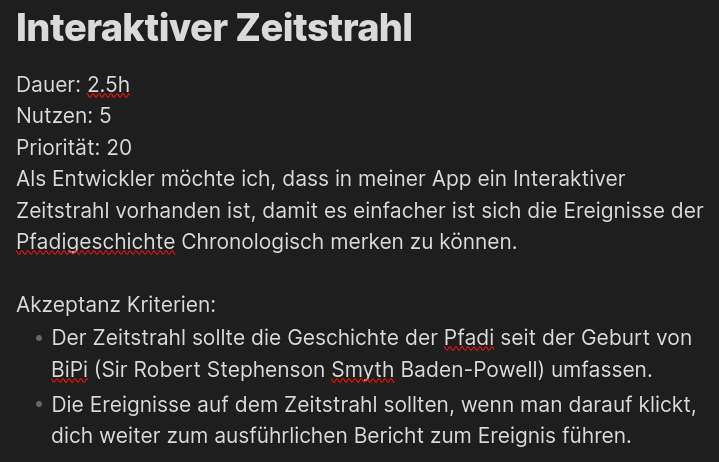
\includegraphics[width=0.49\textwidth]{Picture/Interaktiver Zeitstrahl.png}} &
        \adjustbox{valign=t}{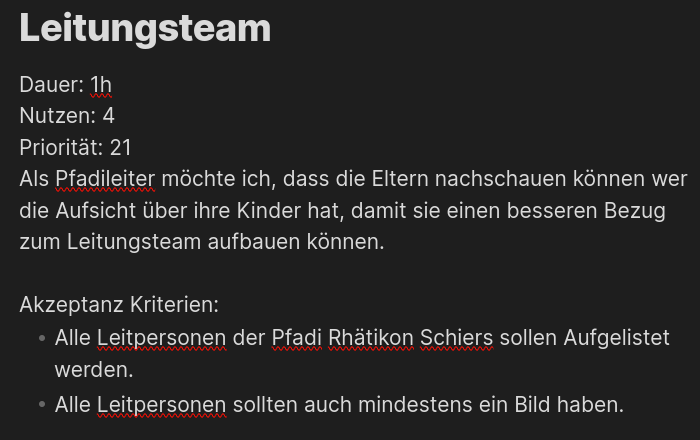
\includegraphics[width=0.49\textwidth]{Picture/Leitungsteam.png}} \\
        \vspace{0.01\textwidth} \\
    \end{tabular}
\end{table}

\begin{table}[ht]
    \centering
    \begin{tabular}{c c}
        \adjustbox{valign=t}{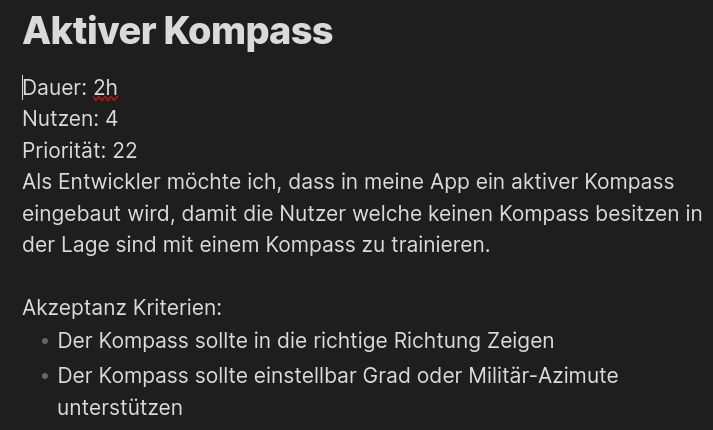
\includegraphics[width=0.49\textwidth]{Picture/Aktiver Kompass.png}} &
        \adjustbox{valign=t}{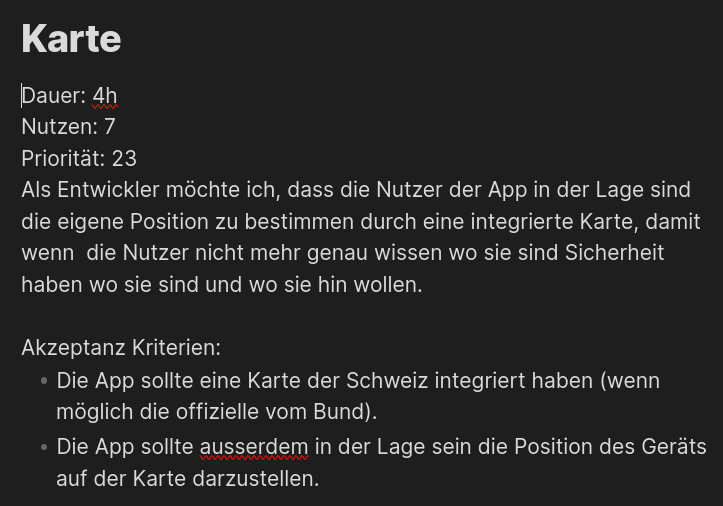
\includegraphics[width=0.49\textwidth]{Picture/Karte.png}} \\
        \vspace{0.01\textwidth} \\
        \adjustbox{valign=t}{\includegraphics[width=0.49\textwidth]{Picture/Seilbünde.png}} &
        \adjustbox{valign=t}{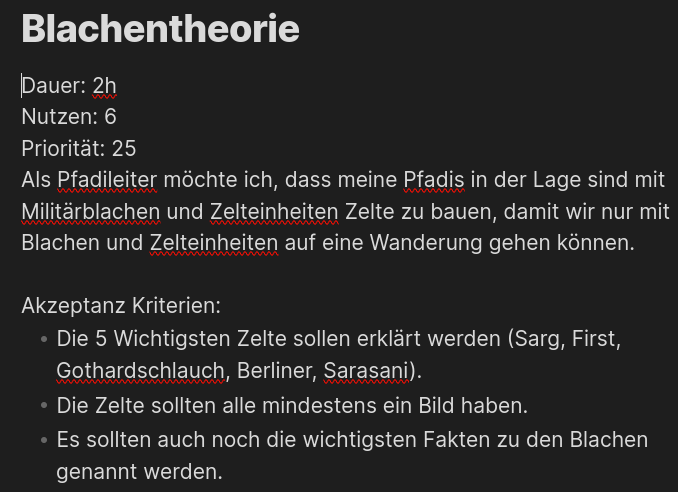
\includegraphics[width=0.49\textwidth]{Picture/Blachentheorie.png}} \\
        \vspace{0.01\textwidth} \\
        \adjustbox{valign=t}{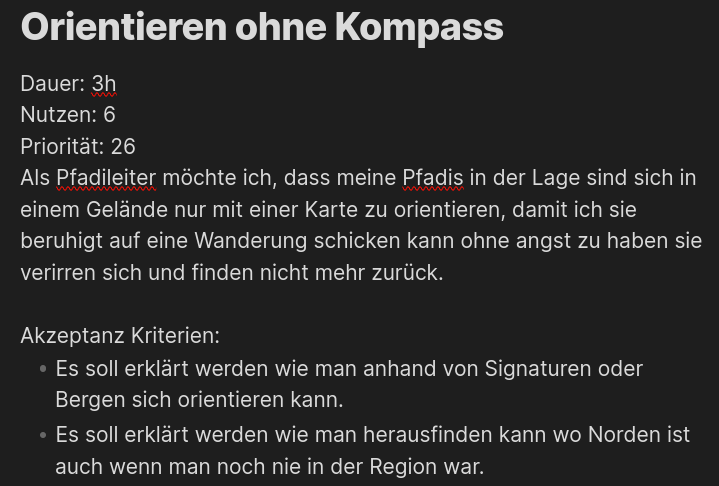
\includegraphics[width=0.49\textwidth]{Picture/Orientieren ohne Kompass.png}} &
        \adjustbox{valign=t}{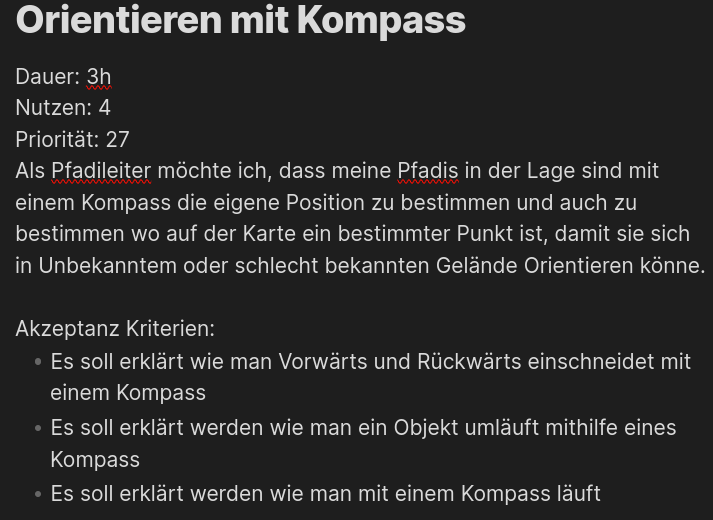
\includegraphics[width=0.49\textwidth]{Picture/Orientieren mit Kompass.png}} \\
        \vspace{0.01\textwidth} \\
\end{tabular}
\end{table}

\begin{table}[ht]
    \centering
    \begin{tabular}{c c}
        \adjustbox{valign=t}{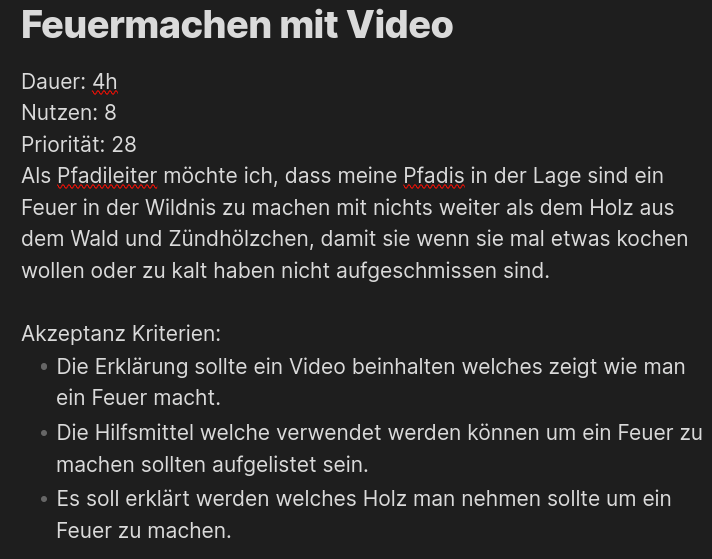
\includegraphics[width=0.49\textwidth]{Picture/Feuermachen mit Video.png}} &
        \adjustbox{valign=t}{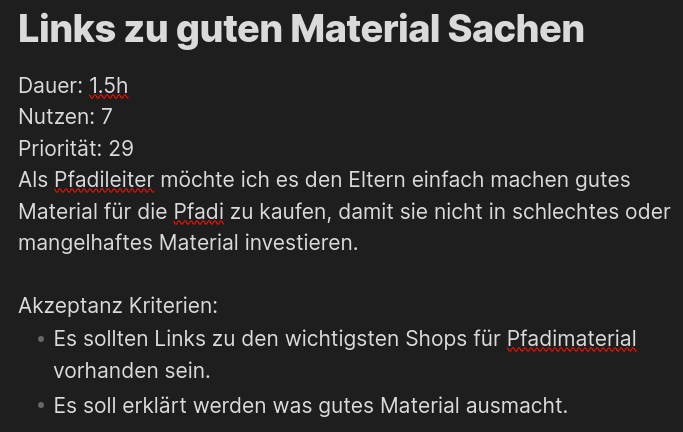
\includegraphics[width=0.49\textwidth]{Picture/Links zu gutem Pfadimaterial.png}} \\
        \vspace{0.01\textwidth} \\
        \adjustbox{valign=t}{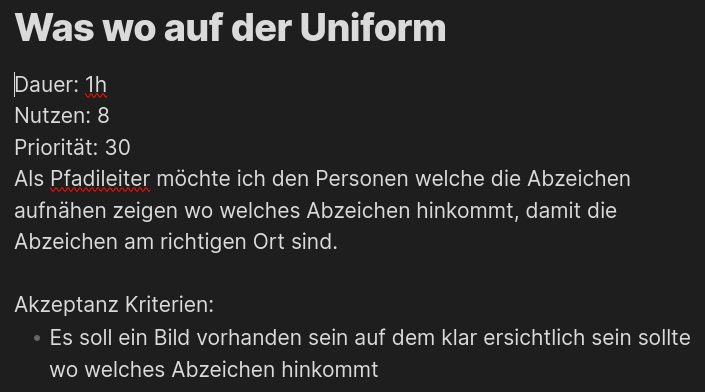
\includegraphics[width=0.49\textwidth]{Picture/Was wo auf der Uniform.png}} &
        \adjustbox{valign=t}{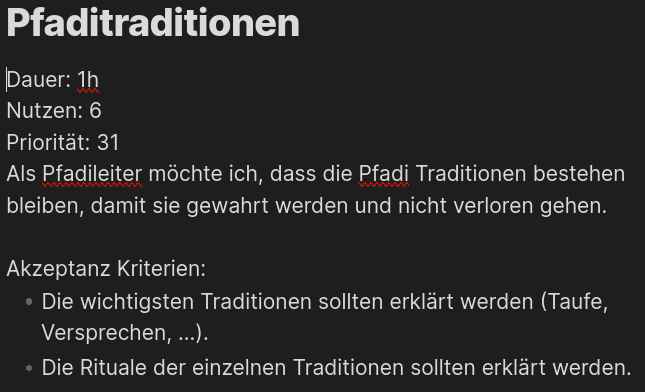
\includegraphics[width=0.49\textwidth]{Picture/Pfaditraditionen.png}} \\
        \vspace{0.01\textwidth} \\
        \adjustbox{valign=t}{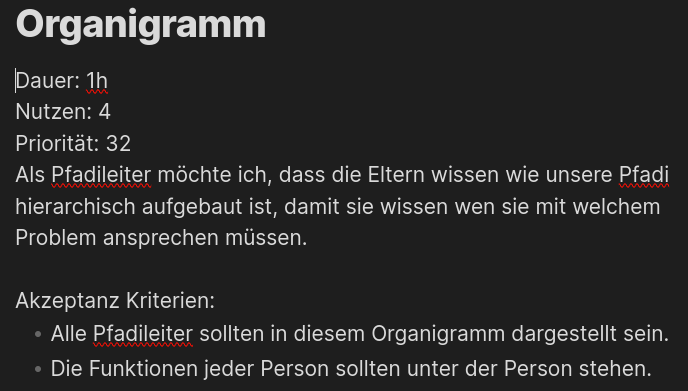
\includegraphics[width=0.49\textwidth]{Picture/Organigramm.png}} &
        \adjustbox{valign=t}{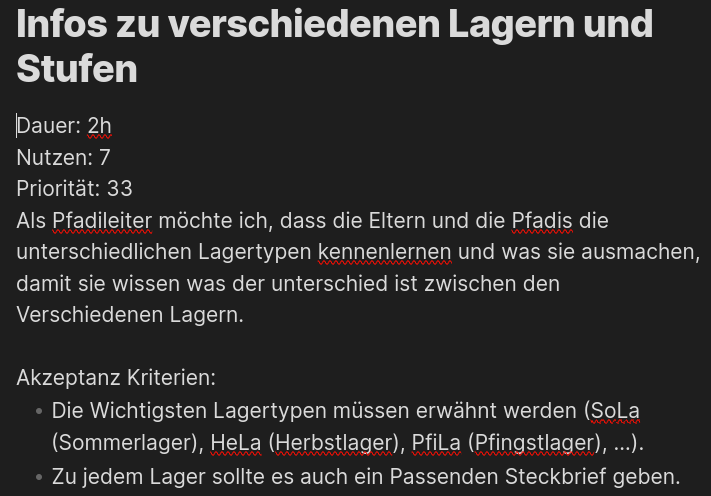
\includegraphics[width=0.49\textwidth]{Picture/Infos zu verschiedenen Lagern und Stufen.png}} \\
        \vspace{0.01\textwidth} \\
        
    \end{tabular}
\end{table}

\begin{table}[ht]
    \centering
    \begin{tabular}{c c}
        \adjustbox{valign=t}{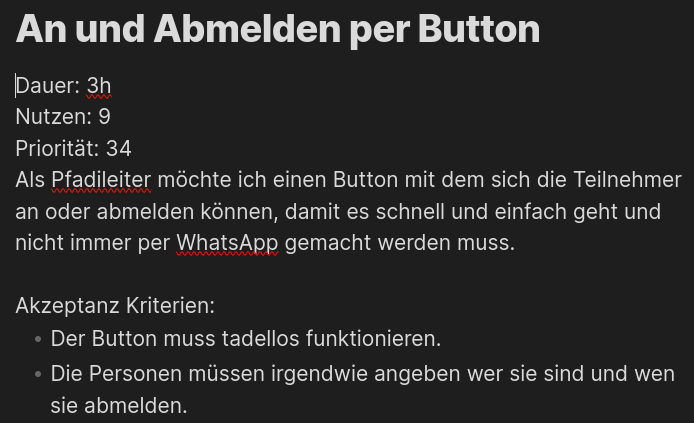
\includegraphics[width=0.49\textwidth]{Picture/An und Abmelden per Button.png}} &
        \adjustbox{valign=t}{\includegraphics[width=0.49\textwidth]{Picture/Kalender mit Aktivitäten.png}} \\
        \vspace{0.01\textwidth} \\
        \adjustbox{valign=t}{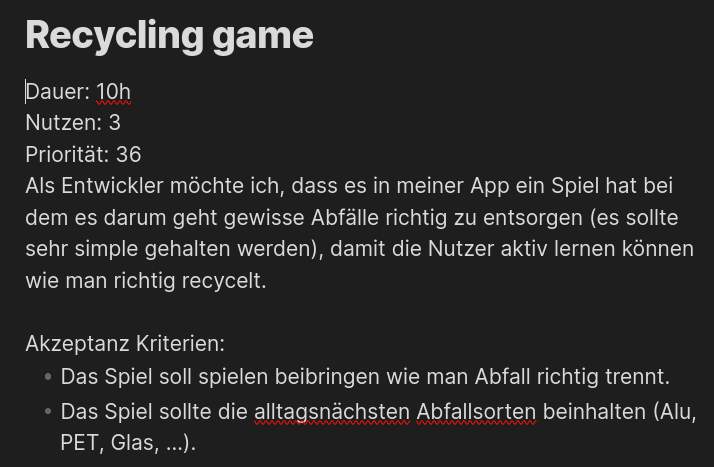
\includegraphics[width=0.49\textwidth]{Picture/Recyclinggame.png}} &
        \adjustbox{valign=t}{\includegraphics[width=0.49\textwidth]{Picture/Chatfunktion für Eltern und Leiter.png}} \\
    \end{tabular}
\end{table}

\clearpage
\section{Test Anfangs und Schlusserhebung des Testlaufs}

\begin{figure}[!h]
    \centering
    \begin{minipage}[t]{0.49\textwidth}
        \centering
        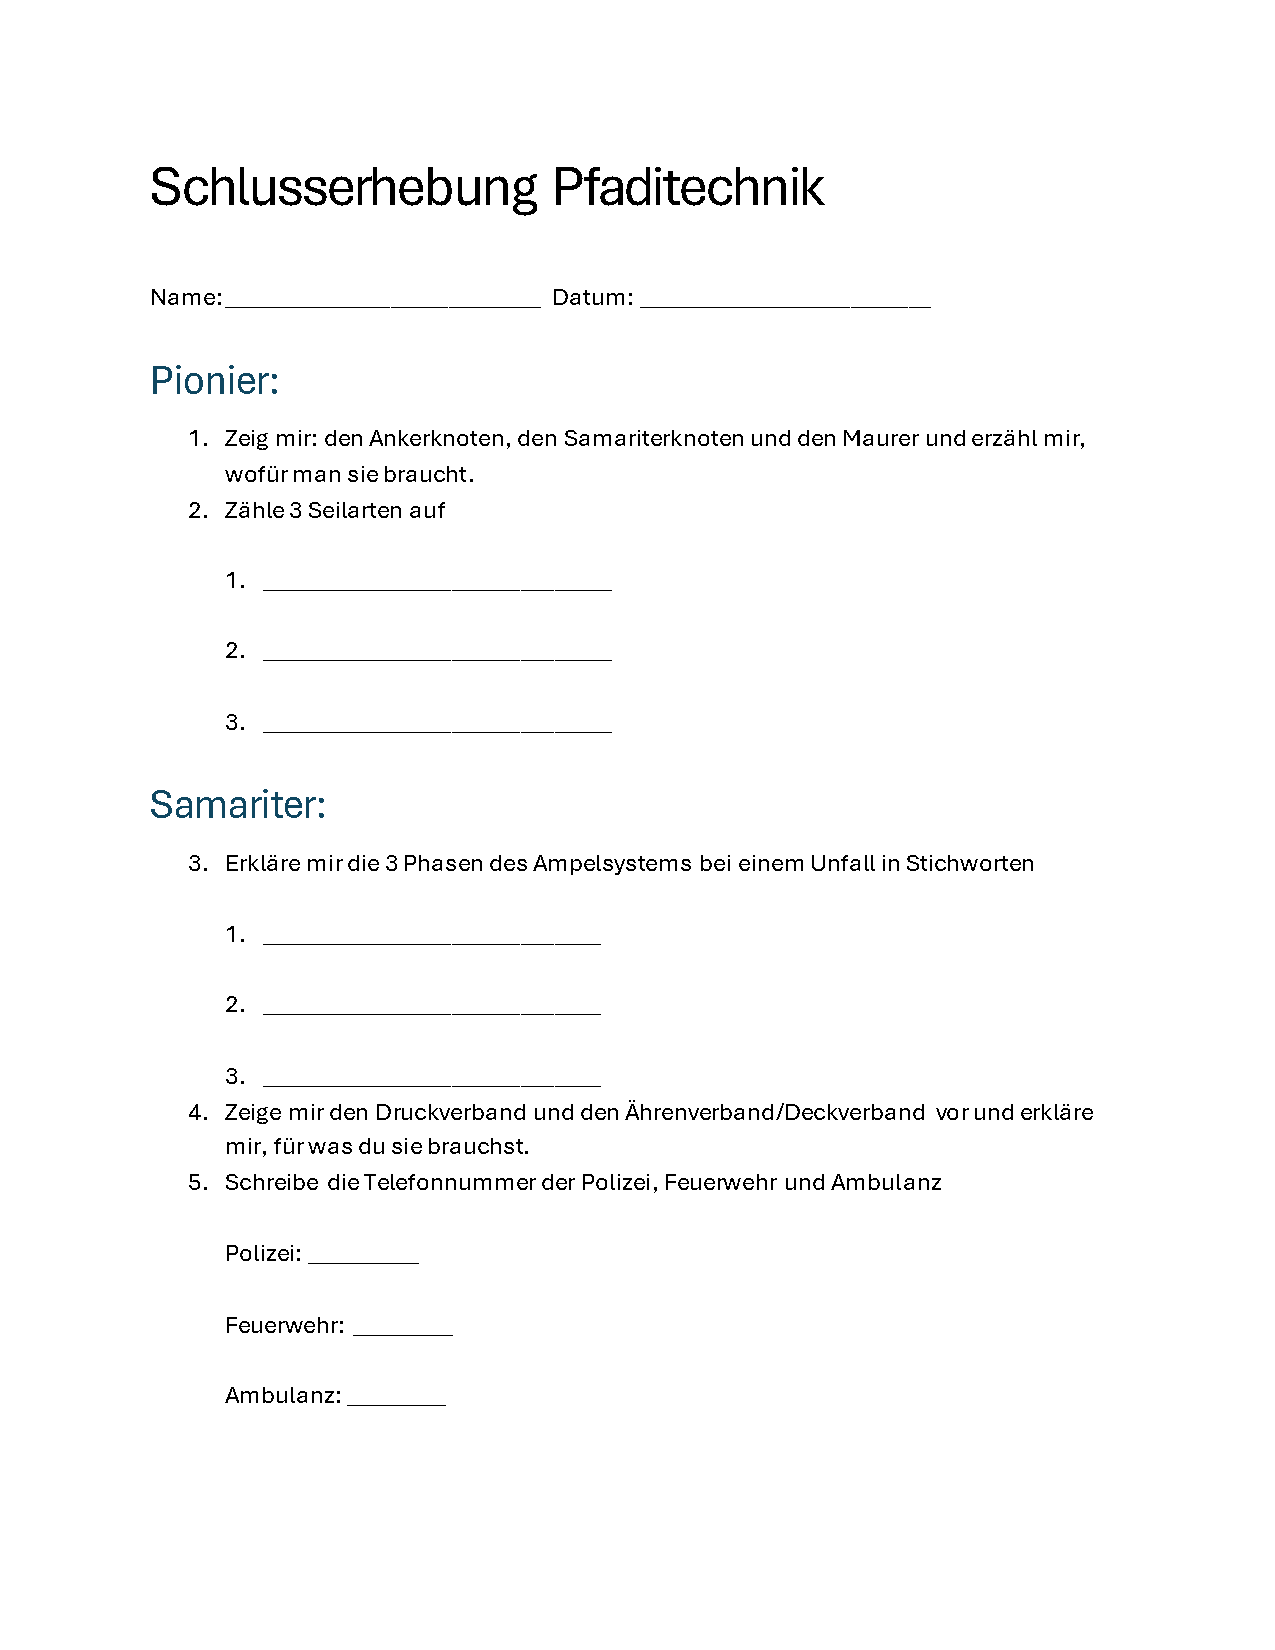
\includegraphics[width=\textwidth]{Picture/seite1.pdf}
    \end{minipage}
    \begin{minipage}[t]{0.49\textwidth}
        \centering
        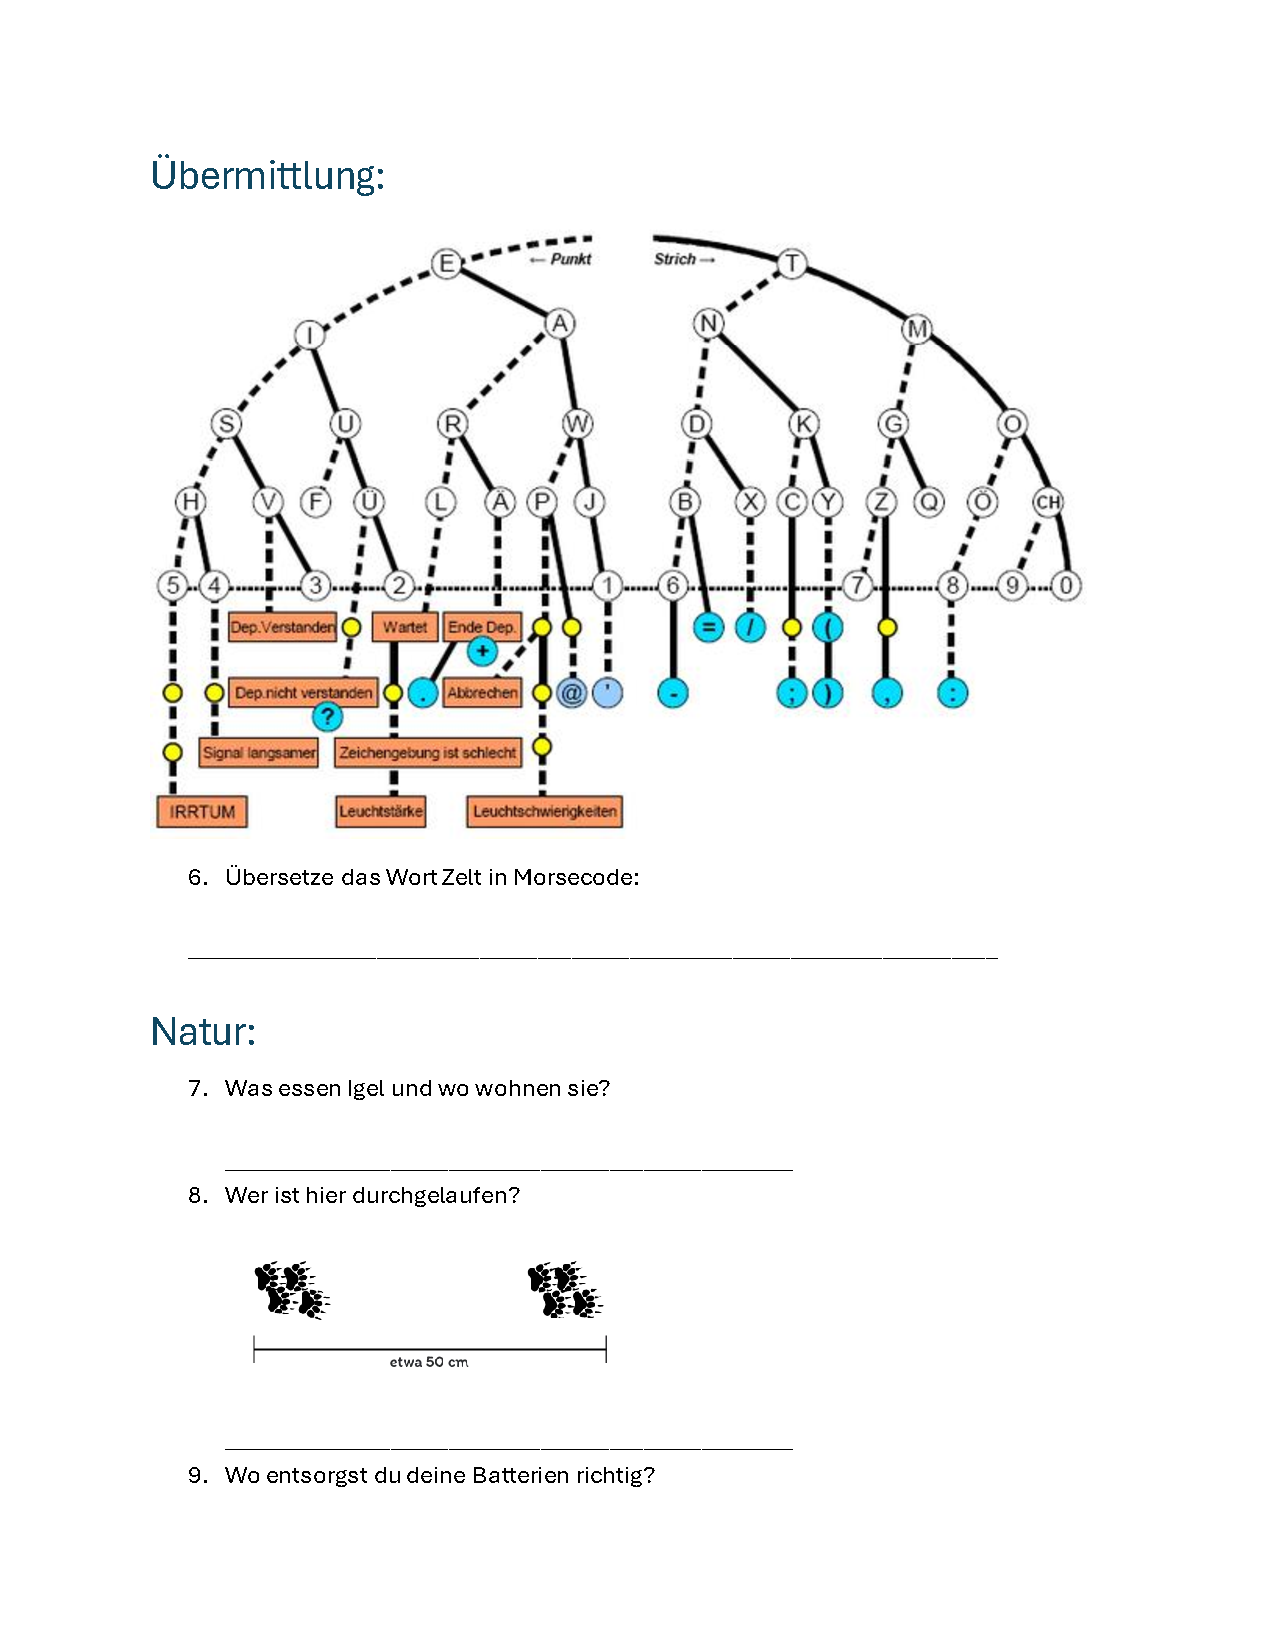
\includegraphics[width=\textwidth]{Picture/seite2.pdf}
    \end{minipage}
    
    \vspace{0.05\textwidth}
    
    \begin{minipage}[t]{0.49\textwidth}
        \centering
        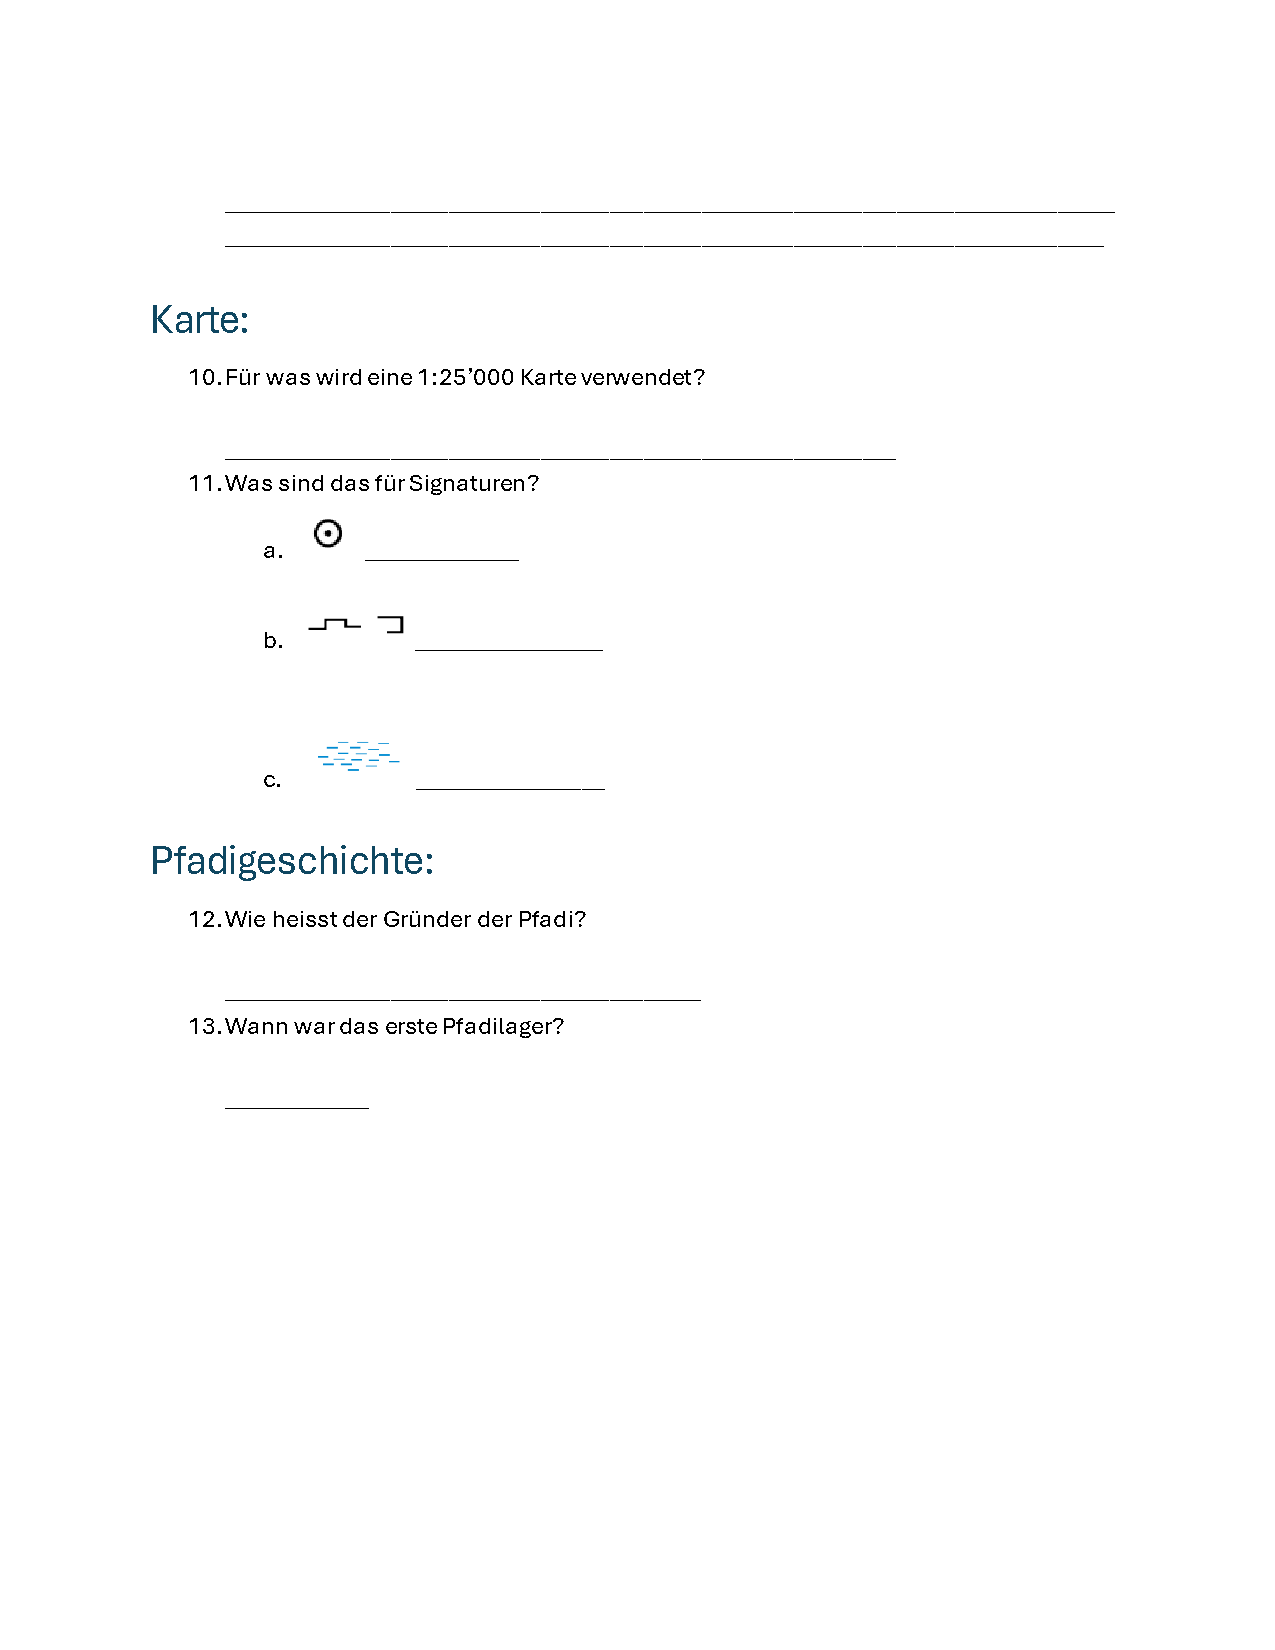
\includegraphics[width=\textwidth]{Picture/seite3.pdf}
    \end{minipage}
    \begin{minipage}[t]{0.49\textwidth}
        \centering
        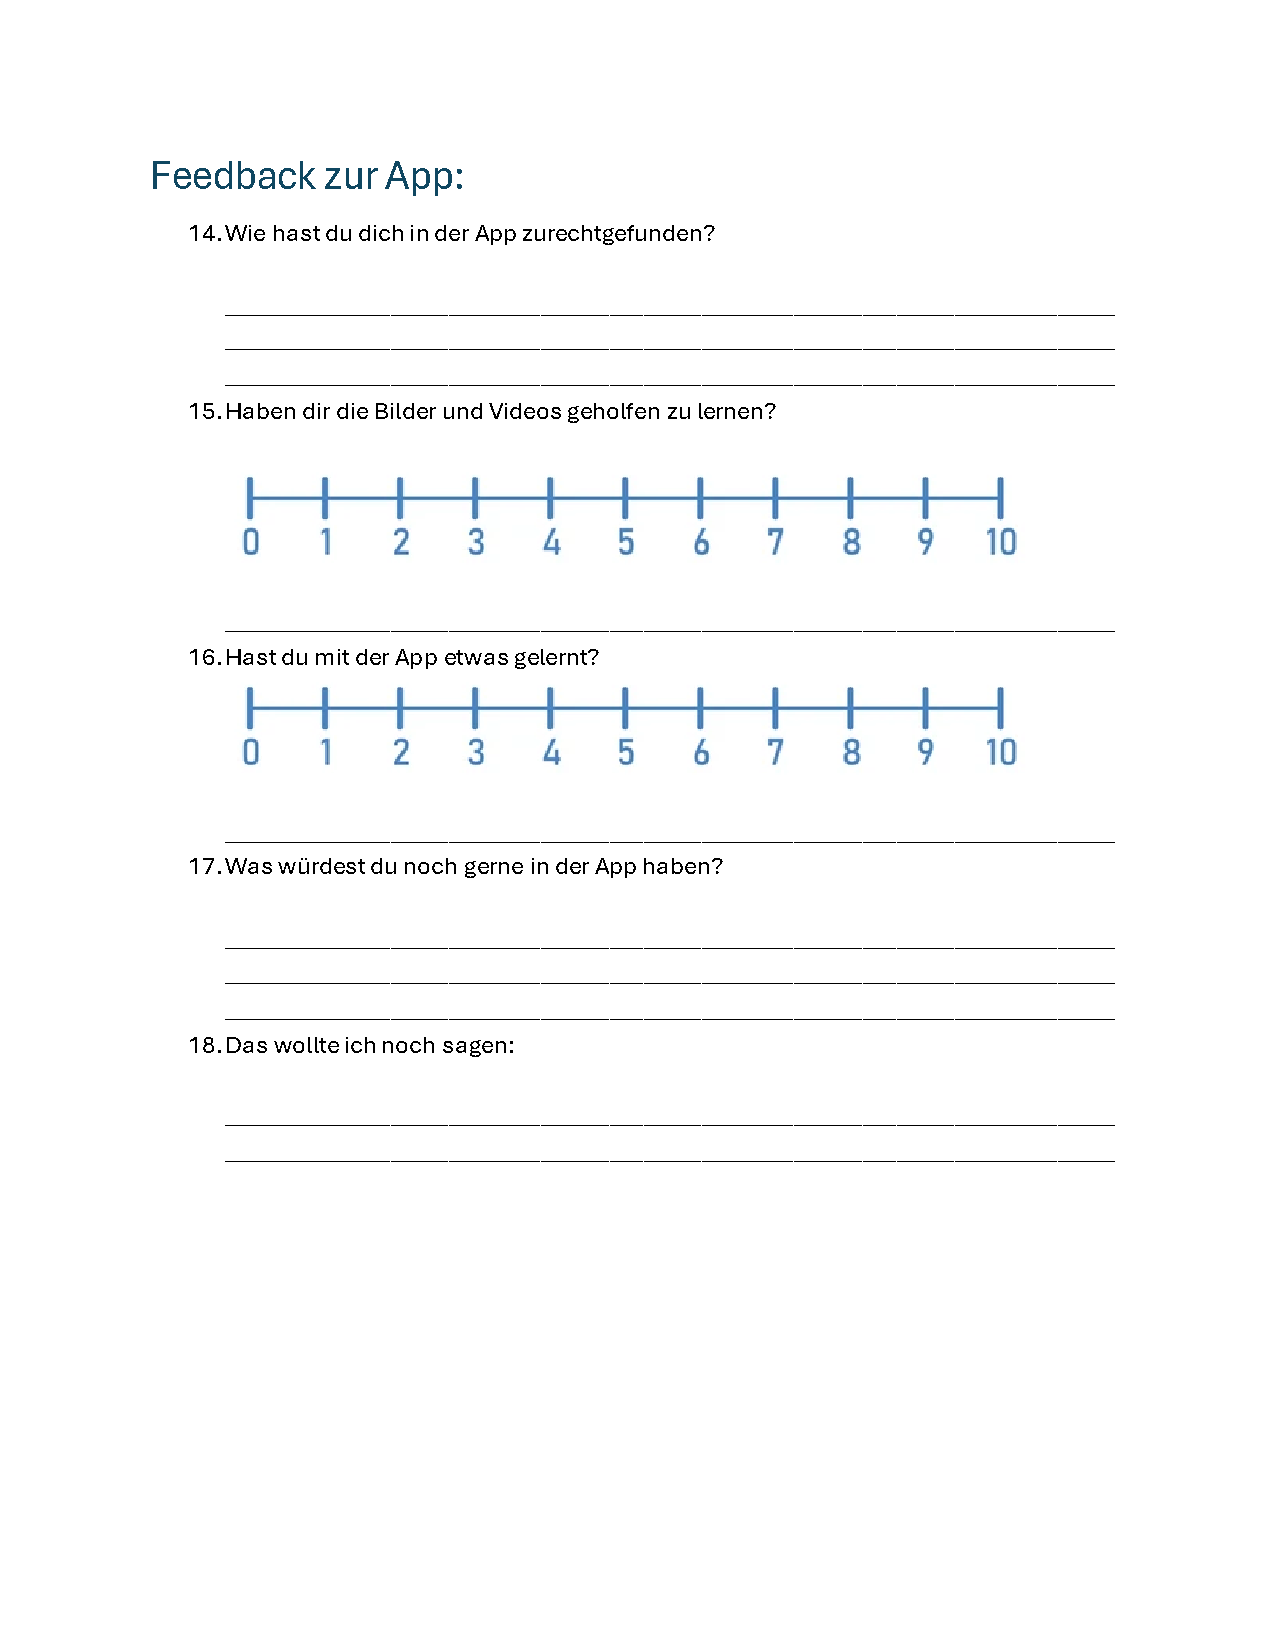
\includegraphics[width=\textwidth]{Picture/seite4.pdf}
    \end{minipage}
\end{figure}

\newpage

\section{Stichprobe Mails}

Dies sind die beiden Mails, die den Eltern geschickt wurden, um sie über App zu informieren für die Stichprobe.
\\\\
\textbf{Email vom 16.9.2024:}
\\\\
Liebe Eltern und Pfadis 
\\\\
Die Etappenprüfungen der Pfadis stehen wieder kurz bevor und die Vorbereitungen dafür laufen auf Hochtouren. Um die Vorbereitung auf die Etappen für euch und euere Kinder ein wenig zu erleichtern, habe ich im Rahmen meiner Maturaarbeit eine Android App programmiert. Mit dieser App kann man das Wissen der ersten Etappe erlernen.  
\\\\
Für meine Maturaarbeit brauche ich Feedback von Leuten, welche die App ausprobiert haben. Hier bin ich auf eure Hilfe angewiesen! Bitte schaut euch die App an oder bereitet euch für die Etappen mit meiner App vor. Nach den Etappen werde ich mich mit einer Umfrage bei euch melden, um euer Feedback abzuholen und Verbesserungsvorschläge zu erhalten, wie ich die App noch besser machen könnte.  
\\\\
Die Datei, um die App herunterzuladen, findet ihr im Anhang. Um die App nutzen zu können, müsst den Button “Apps von diesem Hersteller vertrauen” klicken. Die App funktioniert nur auf Android Geräten und noch nicht auf Apple. 
\\\\
Danke an alle, die sich die Zeit nehmen, sich mit der App auseinandersetzen und mir dazu ein Feedback geben. 
\\\\
Herzliche Grüsse 
\\\\
Munzel v/o Andrea Bardill
\\\\
\textbf{Email vom 23.9.2024:}
\\\\
Liebe Eltern und Pfadis,
\\\\
die Etappenprüfungen liegen nun hinter uns, und ich hoffe, sie waren ein Erfolg für alle! Wie angekündigt, möchte ich mich nun an euch wenden, um euer wertvolles Feedback zur App zu sammeln.
\\\\
Ich hoffe, die App hat euch und euren Kindern bei der Vorbereitung geholfen. Jetzt wäre ich sehr dankbar, wenn ihr euch einen Moment Zeit nehmen könntet, um mir eure Erfahrungen und Eindrücke mitzuteilen. Eure Rückmeldungen sind für mich von grosser Bedeutung, um die App weiter zu verbessern und gegebenenfalls noch benutzerfreundlicher zu gestalten.
\\\\
Im Folgenden findet ihr einen Link zu einer kurzen Umfrage, in der ihr mir Feedback geben könnt:
\\\\
https://forms.gle/q19eWQkpnUJy7iy79
\\\\
Vielen Dank nochmals an alle, die sich die Zeit genommen haben, die App auszuprobieren. Mit euren Rückmeldungen tragt ihr wesentlich dazu bei, dass ich die App optimieren und meine Maturaarbeit erfolgreich abschliessen kann.
\\\\
Ich freue mich auf eure Antworten und danke euch herzlich für eure Unterstützung!
\\\\
Herzliche Grüsse
\\\\
Munzel v/o Andrea Bardill

\section{Quellen}
Die Liste der Quellen, die im Text nie erwähnt werden, aber dennoch dem Projekt geholfen haben. \\
\begin{description}
    \item[Stack Overflow] \url{https://stackoverflow.com/}
    \item[The tabularx package] \url{https://texdoc.org/serve/tabularx/0}
    \item[The Code City] \url{https://www.youtube.com/watch?v=VJOblwM2KJ0}
\end{description}

\section{Abbildungsverzeichnis App}

Die Liste der Bildquellen welche in der App verwendet wurden.\\\\
\sloppy
\noindent
End Achter: \url{https://images.app.goo.gl/PrDLJTNYEkjqFXxVA} \\
Mastwurf: \url{https://de.scoutwiki.org/Achterschlinge} \\
Ampelsystem: \url{https://images.app.goo.gl/LLKyf2hM6ozbSrxq7} \\
Anker: \url{https://images.app.goo.gl/hHbP4AdGtubfDJkG9} \\
Bergseil: \url{https://www.hajk.ch/fr/corde-de-montagne-petzl-mambo-60-m-10-1-mm} \\
BiPi: \url{https://images.app.goo.gl/MhkpjjFn6fcY17XH9} \\
Bertzeli: \url{https://images.app.goo.gl/JrEtE4SAm6aTCeXH9} \\
Caesar: \url{https://images.app.goo.gl/SRohNwMSCLWjqR2FA} \\
Druckverband: \url{https://images.app.goo.gl/75GwTo9HfH8QMEmH9} \\
Druckverband seitlich: \url{https://images.app.goo.gl/5MGtsS3Rx1AKttVk8} \\
Fischer: \url{https://images.app.goo.gl/u1rdZZADAt91ziUF7} \\
Päckli: \url{https://images.app.goo.gl/fpGohozNcUcMcnNJ8} \\
Freimaurer: \url{https://images.app.goo.gl/9pPxFAA871GKedFe8} \\
Händewaschen: \url{https://images.app.goo.gl/JLv3652tbtxfiQQdA} \\
Halbmastwurf: \url{https://images.app.goo.gl/Gi5DpG3u2L2AT4m78} \\
Hamburgerbutton: \url{https://fonts.google.com/icons?icon.size=24&icon.color=%23e8eaed&selected=Material+Symbols+Outlined:menu:FILL@0;wght@400;GRAD@0;opsz@24} \\
Homebutton: \url{https://fonts.google.com/icons?icon.size=24&icon.color=%23e8eaed&selected=Material+Symbols+Outlined:home:FILL@0;wght@400;GRAD@0;opsz@24} \\
Kartenmassstab: \url{https://images.app.goo.gl/4nUr3FW7dfRWJpAY6} \\
Krawattenknopf: \url{https://images.app.goo.gl/FLgnK8FDMrDf1U7D8} \\
Lady Olave: \url{https://images.app.goo.gl/pvtzCLjWsAwgxWPW8} \\
Lilie: \url{https://images.app.goo.gl/FWX3PK3qxv6Htf2E7} \\
Maurer: \url{https://images.app.goo.gl/qbE5sRS1TVaF7xeH7} \\
Tafel Morsen: \url{https://images.app.goo.gl/EFKnZxH5k2nd7b4r7} \\
Morseschlüssel: \url{https://images.app.goo.gl/Xo8oTWq2GoMv4JyJ9} \\
Pfadischiers Logo: \url{https://pfadischiers.ch/about/} \\
Packen: \url{https://images.app.goo.gl/7gvuhbdNJV8ojmy47} \\
Samariter knoten: \url{https://images.app.goo.gl/C97Rwi5QZaDkTZv29} \\
Statikseil: \url{https://images.app.goo.gl/LE7z1qnqLLxsB69g7} \\
Weber: \url{https://images.app.goo.gl/W3SSLaPSFciqj3Nk7} \\
Deckverband: \url{https://images.app.goo.gl/nzw5qP6Z6gPS6dEFA} \\
Signaturen: \url{https://prod-swishop-s3.s3.eu-central-1.amazonaws.com/2024-03/symbols_de.pdf} \\
Amsel: \url{https://images.app.goo.gl/e5FxfFw5xceYFQNo8} \\
Bachstelze: \url{https://images.app.goo.gl/92AkCXqwvqvShi4aA} \\
Dachs: \url{https://images.app.goo.gl/WX6RbbL9Gixh8jS28} \\
Eichhörnchen: \url{https://www.tierchenwelt.de/images/stories/fotos/saeugetiere/nagetiere/eichhoernchen/eichhoernchen_l.jpg} \\
Erdkröte: \url{https://images.app.goo.gl/QvUg6QtD2E3Q8VdR9} \\
Feldhase: \url{https://www.jagdverband.de/sites/default/files/styles/large/public/Rolfes%20Hase%20WR%2011%201820_3x2.jpg?itok=9NGgFpvF} \\
Feldmaus: \url{https://res.cloudinary.com/dewist/image/upload/f_auto,q_70,fl_lossy,w_1200,h_750,c_fill,e_unsharp_mask:90,fl_keep_iptc/v1707640642/media/pages/wildtiere/feldmaus/623e754d02-1707640642/steckbrief_feldmaus-fullscreenheader.jpg} \\
Feuersalamander: \url{https://www.waldwissen.net/assets/wald/tiere/reptilien_amphibien_fische/lwf_feuersalamander_2023/lwf_feuersalamander_2023_salamander.jpg} \\
Fledermaus: \url{https://www.sonova.com/sites/default/files/styles/content_image/public/2019-10/fledermaus_1282913071.jpg?itok=KR8rbKwi} \\
Fuchs: \url{https://upload.wikimedia.org/wikipedia/commons/thumb/b/bc/Vulpes_vulpes_1_%28Martin_Mecnarowski%29.jpg/640px-Vulpes_vulpes_1_%28Martin_Mecnarowski%29.jpg} \\
Gemse: \url{https://upload.wikimedia.org/wikipedia/commons/thumb/f/f0/064_Wild_Chamois_Parc_r%C3%A9gional_Chasseral_Photo_by_Giles_Laurent.jpg/800px-064_Wild_Chamois_Parc_r%C3%A9gional_Chasseral_Photo_by_Giles_Laurent.jpg} \\
Grasfrosch: \url{https://upload.wikimedia.org/wikipedia/commons/thumb/b/be/European_Common_Frog_Rana_temporaria_%28cropped%29.jpg/1200px-European_Common_Frog_Rana_temporaria_%28cropped%29.jpg} \\
Grünfink: \url{https://www.vogelwarte.ch/wp-content/assets/images/bird/artbilder/700px/5330_0.jpg} \\
Grünspecht: \url{https://www.lbv.de/files/user_upload/Bilder/Arten/Tiere/Vogel%20von%20A-Z/Nichtsingvogel/Gruenspecht/Gruenspecht_maennlich-Rosl-Roessner.jpg} \\
Habicht: \url{https://www.lbv.de/files/user_upload/Bilder/Arten/Tiere/Vogel%20von%20A-Z/Greifvogel/Habicht/Habicht_Herbert%20Henderkes.jpg} \\
Igel: \url{https://www.kindernetz.de/wissen/tierlexikon/1653498724688%2Csteckbrief-igel-102~_v-1x1@2dL_-029cdd853d61a51824ed2ee643deeae504b065c1.jpg} \\
Kohlmeise: \url{https://birdlife.at/website/image/ir.attachment/24255_900daa1/datas} \\
Kreuzotter: \url{https://www.rettungsdienst.de/app/uploads/2017/12/Kreuzotter.jpg} \\
Kuckuck: \url{https://www.vogelwarte.ch/wp-content/assets/images/bird/artbilder/700px/3040_0.jpg} \newpage
\noindent
Maulwurf: \url{https://www.ardalpha.de/wissen/natur/tiere/maulwurf-steckbrief-lebens\\weise-gaenge-100~_v-img__16__9__xl_-d31c35f8186ebeb80b0cd843a7c267a0e0c81647.jpg?version=42c71} \\
Mäusebussard: \url{https://www.vogelwarte.ch/wp-content/uploads/2023/04/1150_0.jpg} \\
Murmeltier: \url{https://www.br.de/kinder/murmeltier-im-gebirge-100~_v-img__16__9__xl_-d31c35f8186ebeb80b0cd843a7c267a0e0c81647.jpg?version=c2390} \\
Reh: \url{https://image.brigitte.de/12241082/t/XW/v2/w1440/r1.5/-/krafttier-reh-teaser.jpg} \\
Ringelnatter: \url{https://lh3.googleusercontent.com/proxy/E3_FpGr74hb5lv0JKQqdyilw5bHENXtHhCrm5MRBVkqOpgX8OSHmwNrYwqqO1uz018uYE4sL9aG2dVN9kG\\9PDaSOXTTBOEPanwpaFUArXLjvuCJVIy4AR_ppQckR} \\
Rothirsch: \url{https://www.nabu.de/imperia/md/nabu/images/arten/tiere/saeugetiere/paarhufer/190816_rothirsch_nabu-marc_scharping_680x453.png} \\
Rotmilan: \url{https://upload.wikimedia.org/wikipedia/commons/thumb/4/4b/Milvus_milvus_R%28ThKraft%29.jpg/300px-Milvus_milvus_R%28ThKraft%29.jpg} \\
Spitzmaus: \url{https://www.mpg.de/11667277/original-1664362311.jpg?t=eyJ3aWR0aCI6MTIwMCwiaGVpZ2h0Ijo2MjgsImZpdCI6ImNyb3AiLCJvYmpfaWQiOjExNjY3Mjc3fQ%3D%3D--ff01429b0f598ed66e011cb435bb047c263f4985} \\
Steinbock: \url{https://www.passionedolomiti.com/wp-content/uploads/2019/12/ibex-3852432_1280.jpg} \\
Steinmarder: \url{https://www.sbs.sachsen.de/img/Steinmarder_rdax_87s.jpg} \\
Turmfalke: \url{https://www.nabu.de/imperia/md/nabu/images/arten/tiere/voegel/falken/161220-nabu-turmfalke-hartmut-mletzko.jpeg} \\
Uhu: \url{https://www.lbv.de/assets/images/d/Uhu%20-%20%20Sturm%20Ralph_LBV%20Bildarchiv1-cf8bb12d.webp} \\
Waldkauz: \url{https://www.nabu.de/imperia/md/nabu/images/arten/tiere/voegel/eulen/20140812-nabu-waldkauz-tom-dove.jpeg} \\
Tierspuren: \url{https://naturpark-detektive.de/wiki-eintrag/tierspuren/} \\
Recycling: \url{https://corporate.migros.ch/de/verantwortung/nachhaltigkeit/verpackung-und-recycling/recycling-guide} \\